\documentclass[a4paper,11pt]{article}
\usepackage[utf8]{inputenc}
\usepackage[francais]{babel}
\usepackage{graphicx}
\usepackage{fancyhdr}
\usepackage {color}
\usepackage{colortbl}
\usepackage{hyperref}
\usepackage{listings}
\lstset{basicstyle=\footnotesize\ttfamily,breaklines=true}
% Title Page
\title{SPAM ASSASSIN}
\date{Décembre 2014}
\author{Mathieu KERN - Aymeric HINDERCHIETTE}
\pagestyle{fancy}


\begin{document}

\maketitle
\includegraphics{spamassassinintro.png}
\pagebreak

\tableofcontents

\pagebreak

\part{Présentation de SpamAssassin}

\section{Problématique }

  Le mail (ou courriel) est aujourd'hui le moyen privilégié de communication à travers le monde. Massivement utilisé, 
d'une certaine fiabilité et éprouvé par des décennies d'utilisation il reste le moyen le plus répandu pour 
les communications entres les personnes. Malheureusement, mail est également aujourd'hui synonyme de spam, ces messages
indésirables qui s'entassent dans nos boites mails. C'est ici qu'entre en jeu SpamAssassin.

\subsection{Le SPAM}
Avant de poursuivre sur SpamAssassin, rappelons concrètement ce qu'est le SPAM et ce qu'il implique. 

\paragraph{Comment reconnaître un SPAM:}

\begin{itemize}
 \item De par sa nature, un SPAM n'est pas désiré par l'utilisateur qui le reçoit. 
 \item La réception d'un SPAM résulte d'un envoi massif: une machine (souvent un bot) envoie le même message 
 à plusieurs destinataires sans aucun discernement. Cela s'oppose aux messages ciblés par exemple de commerçant,
 qui n’envoie que à leurs prospects (à but publicitaire ou informatif).
 \item Son contenu n'est pas destiné spécifiquement à l'utilisateur (chaque personne reçoit le même contenu).
 \item Une importante liste de destinataires.
 \item Entête des messages souvent corrompues ou ne respectant pas les normes.
\end{itemize}

\paragraph{Statut légal}


La loi pour la confiance dans l'économie numérique du 21 juin 2004 contient une transposition de la
directive européenne du 12 juillet 2002\footnote{Le principe introduit figurera également à l'article L.34.5 du code 
des postes et des communications électroniques } relative à la protection de la vie privée dans le secteur des communications
électroniques:
\begin{quote}
 Est interdite la prospection directe au moyen d'un automate d'appel, d'un télécopieur ou d'un courrier électronique utilisant,
 sous quelque forme que ce soit, les coordonnées d'une personne physique qui n'a pas exprimé son consentement préalable à recevoir
 des prospections directes par ce moyen. 
\end{quote}
Les SPAM sont donc connus du droit français et encadrés par des textes spécifiques.

\section{Le projet}

\subsection{Informations}


\begin{center}
\begin{tabular}{cll}
\hline
Développeur & Apache Software Foundation  \\
Langage & Perl 
Dernière version & 3.4.0 (11 février 2014) [+/-] \\
Environnements & Multiplate-forme  \\
Type & Anti-spam & \\
Licence & Licence Apache 2.0 \\ \\
\hline
\end{tabular}
\end{center}



SpamAsassin est donc aujourd'hui sous le giron de la Apache Software Foundation, organisation à but non lucratif qui
s'occupe également du serveur Apache, Logiciel de distribution de contenu WEB le plus utilisés au monde. 
Elle gère également 150 autres projets.

\paragraph{La licence apache}
En outre tout ses projets sont distribués sous sa propre Licence, la licence Apache(actuellement en 2.0) , qui est compatible GPL v3.
Cette licence met l’accent sur le copyright tout en restant bien sur une licence libre. Les objectifs principaux de la Fondation sont de protéger 
juridiquement le travail des contributeurs et d'empêcher que la marque Apache soit utilisée illégalement.

Le projet SpamAssassin est actif depuis plus d'une décennie et est constamment en développement 
pour s'adapter aux développements des méthodes qu'utilisent les spammeurs. C'est en outre le programme anti-spam le plus utilisé à cause de son efficacité.

\subsection{Développement}

SpamAssasin contient environ 300 000 lignes de codes ce qui en fait un très gros projet( Graphique ~\ref{fig:code}).
Le projet est à maturité et il ne grossit plus depuis plusieurs années, les développeurs se concentrant sur l'optimisation du code existant.

Il y actuellement 23 développeurs principaux, avec une répartition des lignes codes assez inégales, notamment deux développeurs qui ont fait la majorité du code( Tableau ~\ref{tab:devs}).
Mais vu que c'est un projet libre et open source, chacun est libre de contribuer et forker le projet. Cela concerne aussi 
bien les particuliers que les entreprises (En respectant bien sur les restrictions de la licence Apache).

\begin{figure}[h]
 \includegraphics[width=\textwidth]{annexes/lignes.png}
  \caption{Évolution du nombre de ligne de codes}
  \label {fig:code}
\end{figure}

\begin{table}[ht]!
 
\definecolor{tcA}{rgb}{0.627451,0.627451,0.643137}
\begin{center}
\begin{tabular}{lllll}

\rowcolor{tcA}
 Author Id & Changes & Lines of Code & Lines per Change\\
\rowcolor{tcA}
 Totals & 26092 (100.0\%) & 1403447 (100.0\%) & 53.7\\
\rowcolor{tcA}
  jm & 8136 (31.2\%) & 721593 (51.4\%) & 88.6\\
\rowcolor{tcA}
  spamassassin role & 7997 (30.6\%) & 463448 (33.0\%) & 57.9\\
\rowcolor{tcA}
  axb & 741 (2.8\%) & 54525 (3.9\%) & 73.5\\
\rowcolor{tcA}
  mmartinec & 1779 (6.8\%) & 32348 (2.3\%) & 18.1\\
\rowcolor{tcA}
  felicity & 1625 (6.2\%) & 29134 (2.1\%) & 17.9\\
\rowcolor{tcA}
  kmcgrail & 605 (2.3\%) & 21294 (1.5\%) & 35.1\\
\rowcolor{tcA}
  quinlan & 1100 (4.2\%) & 19583 (1.4\%) & 17.8\\
\rowcolor{tcA}
  parker & 309 (1.2\%) & 10407 (0.7\%) & 33.6\\
\rowcolor{tcA}
  khopesh & 1369 (5.2\%) & 10296 (0.7\%) & 7.5\\
\rowcolor{tcA}
  dos & 427 (1.6\%) & 8427 (0.6\%) & 19.7\\
\rowcolor{tcA}
  jhardin & 1021 (3.9) & 6845 (0.5\%) & 6.7\\
\rowcolor{tcA}
  wtogami & 137 (0.5\%) & 6470 (0.5\%) & 47.2\\
\rowcolor{tcA}
  hstern & 63 (0.2\%) & 6029 (0.4\%) & 95.6\\
\rowcolor{tcA}
  sidney & 275 (1.1\%) & 3552 (0.3\%) & 12.9\\
\rowcolor{tcA}
  jquinn & 28 (0.1\%) & 2181 (0.2\%) & 77.8\\
\rowcolor{tcA}
  mss & 133 (0.5\%) & 2072 (0.1\%) & 15.5\\
\rowcolor{tcA}
 hege & 95 (0.4\%) & 1931 (0.1\%) & 20.3\\
\rowcolor{tcA}
 duncf & 109 (0.4\%) & 1892 (0.1\%) & 17.3\\
\rowcolor{tcA}
  jgmyers & 66 (0.3\%) & 508 (0.0\%) & 7.6\\
\rowcolor{tcA}
  smf & 35 (0.1\%) & 499 (0.0\%) & 14.2\\
\rowcolor{tcA}
  maddoc & 11 (0.0\%) & 319 (0.0\%) & 29.0\\
\rowcolor{tcA}
  fanf & 12 (0.0\%) & 49 (0.0\%) & 4.0\\
\rowcolor{tcA}
  kb & 19 (0.1\%) & 45 (0.0\%) & 2.3
\end{tabular}
\caption{Statistique des développeurs du projets }
\footnotesize{Source \footnote{Tableau généré avec StatSVN à partir des sources de SpamAssassin}}
\label{tab:devs}
\end{center}
\end{table}


\subsection{Qu'est ce que SpamAssassin}

SpamAssassin est un programme écrit en PERL dont le but est de filtrer activement les Emails en se basant sur des mécanismes internes. 
SpamAssassin n'effectue aucune action envers les mails, il ajoute seulement des informations personnalisés
qui peuvent être utilisée par d'autres programmes pour effectuer des actions sur les mails (les ranger des dossiers distincts, les supprimer, les bloquer, \dots)


Il peut être utilisé de plusieurs manières:
\begin{itemize}
 \item En mode client, lancé à chaque fois que l'on fait appel à lui
 \item En mode demon grâce à \emph{spamd} , les appels au demon étant fait avec l'utilitaire \emph{spamc}.
 \item Comme une interface de programation: des programmes qui nécessitent des fonctionnalités de filtrage de SPAM peuvent s'interfacer avec SpamAssin
 pour construire des solutions utilisant ses fonctionnalités
\end{itemize}

\pagebreak

\part{Ses fonctionnalités}

\section{Comment il filtre}

SpamAssassin reçoit des mails que lui redirigent d'autres programmes, y effectue des tests pour déterminer si ce sont des SPAMS, 
puis renvoie les mails testés au programme qui les as envoyés.

\paragraph{Les test de SpamAssassin }

\begin{description}
 \item [Champs d'entête] En se basant sur la forme des entêtes et en les comparant avec des schéma connus par SpamAssasin. En effet 
 on peut se base sur la façon dont certains systèmes de SPAMs construisent leurs messages pour les filtrer. 
 \item [Corps du message] Bien sur SpamAssasin permet de filtrer les mails suivant les mots et expressions qu'ils contiennent. 
 ``ceci n'est pas un SPAM'', ``Bonjour je suis une princesse d'un royaume africain'', ``Venez chechez votre lot'', \dots sont des expressions
 typiques pour des SPAMs. 
 \item [Filtre bayésien(détail plus loin ~\ref{baye})] Filtrer les entêtes et le corps d'un message résultera toujours en de multiples faux positifs. C'est ici que le filtrage 
 bayésien se révèle intéressant car il va prendre en considération ce que l'on considère comme SPAM et non SPAM soit des ``bon mails'' (``HAM'' en anglais).
 Il va ensuite utiliser les répertoires de SPAMs connu et de ``HAM``  connus, pour y identifier les mots et phrases (Définits comme ''Tokens`` en anglais)
 qui n'apparaissent que dans les SPAMs et que dans les ''HAMs``.
 Un token SPAM trouvé résultant d'une hausse du score (voir \ref{score}) SPAM, un token résultant en une baisse de ce niveau. Ce filtrage permet d'être plus précis et d'éviter les faux positifs, 
 en ne se basant pas juste sur un mot ou une phrase mais des ensembles. 
 \item [List noire/blanche automatique] SpamAssassin garde automatiquement une liste blanches des expéditeurs des mails.
 Pour chaque nouveau mail le programme compare le mail précédent provenant de la même adresse mail et adresse IP.
 Comme précédemment si une adresse email a envoyé un SPAM, ce nouveau mail verra son score augmenté. A l'inverse si c'était un bon mail son score 
 se verra baisser.
 \item [Liste noire/blanche manuelle] Il est tout à fait possible de définir ses propres listes, en autorisant ou 
 interdisant des mails de certaines adresses
 \item [Signalements] En utilisant des signatures établis à partir de mails signalés par les utilisateurs. Il y a notamment les projets DCC, Pyzor, et Razor2
 qui possèdent des bases de données de mails signalés comme SPAM. SpamAssassin va ainsi demander à ces bases si les mails qu'il reçoit 
 sont présents dans leurs donnée.
 \item [DNS blocklists] Ce sont des des bases de données contenant des adresses IP signalées comme expédiant du SPAM ou mal 
 configurée(Par exemple en étant un relais ouvert). Également sont pris en compte les IP de particuliers (considérant qu'il y a peu de chance
qu'un particulier envois directement des mails sans passer par son FAI. Ces signalements vont être pris en compte par SpamAsassin pour le score des mails.
Il intègre nativement quelque une de ces listes.
\item [Caractères et langues] on peut spécifier des caractères et langues comme SPAM.

C'est ces ensembles de règles qui fonctionnant conjointement permettent à SpamAssassin de garantir un haut 
niveau de fiabilité de détection des SPAM, un test pouvant ne pas fonctionner mais sera contrebalancé par les autres.
 \end{description} 


Spam Assassin effectue sur chaque mail qui lui est donné à traiter une série de test, qui vont ensuite donner lieu à un score, qui sera indiqué dans un entête 
si il est considéré comme SPAM. 
Ce résultat sera ensuite utilisé par d'autres programmes pour déterminer des actions à entreprendre.


\section{Le score} \label{score}
C'est la base du signalement des SPAM de SpamAsassin. Un mail après avoir subi des test différents se voit attribuer une note. Cette note permet
ensuite de définir des actions à effectue. Quand un mail est considéré comme SPAM, SpamAssassin ajoute ses propres entêtes (Exemple ~\ref{fig:ex_score}):
\begin{itemize}
 \item ''-Spam-Level: \*\*\*\*\*\*\*\*\* '': Renseigne le score (ici 9)
 \item -Spam-Status: Yes, score=9.0 required=5.0 tests=BAYES\_99,FROM\_EXCESS\_BASE64,FR\_HOWTOUNSUBSCRIBE,FR\_SPAMISLEGAL \dots : Indique des informations relatives aux test effectués et la configuration)
\end{itemize}
. L'utilisateur peut paramétrer ce score pour définir une marge de définitions des SPAMs(valeurs ''require``). Une fois ce score ateint le mail est considéré comme SPAM.
C'est ensuite aux autres programmes d'utiliser ces données. Par exemple on pourrait configurer un MUA pour qu'il sépare 
les SPAM par score suivant des filtres définit. 

\label{baye}

\subsection{Apprentissage}

\subsection{Le filtre bayésien}

Une fonctionnalité qui est une des plus importantes caractéristiques de SpamAssassin est sans doute son filtre
bayésien\footnote{\href {https://fr.wikipedia.org/wiki/Th\%C3\%A9or\%C3\%A8me\_de_Bayes}{Théorème de Bayes}}.
Il va permettre d'établir une connaissance des éléments qui constituent un SPAM et ceux qui n'en sont pas.
\paragraph{Utilisation par SpamAssassin}

Comme annoncé plus haut, ce type de filtre fait partis de son arsenal de test anti-spam. Il va effectuer des tests 
en utilisant les algorithmes de Bayes pour tester des mots et expressions(des''Tokens``), et baisser le score globale du mail si des tokens SPAM sont trouvés. 
A l'inverse si des des tokens ''HAM`` (devant se trouver dans de bon mail) sont trouvés il va abaisser le score du mail, ce qui peut résulter en
des score négatifs.
\linebreak

\paragraph{Sa learn}\footnote{\href{https://spamassassin.apache.org/full/3.1.x/doc/sa-learn.html}{Documentation de sa learn}}
Mais ce que permet surtout ce filtre c'est d'apprendre. En effet il va s'adapter aux utilisateurs. Les utilisateurs
peuvent déclarer un courrier comme SPAM ou ''HAM'' et il sera alors pris en compte par le filtre bayésien de SpamAssasin.
Le programme s'utilise de cette manière:
\begin{itemize}
 \item sa-learn --spam /Chemin/du dossier
 \item sa-learn --ham /Chemin/dudossier
\end{itemize}
Il faut pour garantir l'efficacité et coller aux besoins des utilisateurs que les mails soient ceux de l’utilisateur 
et représentatif de ce qu'il reçoit régulièrement. En outre pour garantir le meilleur taux de réussite
dans la découverte de SPAM, il faut lui faire apprendre plusieurs milliers de mails. Ainsi C'est aux utilisateurs de définir 
ce qu'ils considèrent comme SPAM et non spam. 
\linebreak
Par défaut les tokens sont stockées dans le répertoire des utilisateurs. Pour définir le filtre pour ensembles utilisateurs il faut ajouter 
au \emph{local.cf}:
\begin{lstlisting}[frame=single]
bayes\_path /var/spamassassin/bayes\_db/bayes
bayes\_file\_mode 0777}
\end{lstlisting}
Il faudra veiller à ce que sa-learn puisse régulièrement apprendre les mails des utilisateurs (en l'intégrant par exemple dans un script lancé régulièrement).
\linebreak
Les tokens que génère sa-learn sont stockés dans des bases de données, qui sont par défaut distincte pour chaque utilisateur. Ces Dernière pour éviter de devenir 
trop volumineuse intègre des mécanismes qui régulièrement vont éliminer des tokens inutiles. On peut également en enlever manuellement.
La directive \emph{bayes\_expiry\_max\_db\_size} peut être ajoutée au fichier de configuration générale 
\emph{local.cf} pour définir une limite du nombre de tokens gardés dans la base(par défaut limité à 150 000tokens).
\linebreak
Sa-learn nous permet egalement un export de ces bases (avec l'option --backup du programme sa-learn, en redirigeant la sortie standard),. La restauration se fait 
avec l'option --restore. 
\paragraph*{Auto learning}
Si on ne possède pas de messages stockés à faire apprendre à SpamAssassin , la fonctionnalité \emph{autolearning}
va permettre d'apprendre automatiquement les SPAMs et non SPAMs. Elle est activé par défaut. La masse de mail 
reçu déterminera quand les règles du filtre bayésiens s'activeront(Elle ne peuvent s'activer tant qu'un certains nombre de mails aient été traités par sa-learn).



\section{Articulation du programme}

\subsection{Configuration générale}



La configuration de Spamassassin se fait principalement à travers le fichier \emph{local.cf}(exemple ~\ref{fig:local_sample}), qui se trouve dans le 
répertoire '\emph{/etc/spamassassin}.
Les utilisateurs UNIX peuvent également avoir leurs propres configurations grâce au fichier \emph{user\_prefs}
qui se trouve dans le répertoire \emph{.spamassassin} de leurs home respectifs. 
Par défaut, un certain nombre d’options sont prédéfinies. 
\linebreak
SpamAssassin tient ses avantages en terme de modularité et de sa facilité d'intégration avec d'autres programme de son langage, PERL.
C'est un module PERL qui permet d'être utiliser plus facilement à travers une distributions PERL. 

\subsubsection{Options les plus utilisés}
\paragraph{Désactiver les configurations des utilisateurs}
Dans certains cas on peut désactiver les fichiers de préférences des utilisateurs. Si les utilisateurs n'ont pas accès à leurs configurations 
(pour éviter de lire inutilement les fichiers) ou si SpamAssassin n'est pas appelé par les utilisateurs(dans le cas d'un filtrage générale).

\begin{description}
 \item [Désactiver les préférences utilisateurs]Dans \emph{/etc/default/spamassassin}, il faut changer la ligne d'options pour désactiver les préférences par utilisateur (qui serait normalement stockées dans leur home directory) et utiliser les préférences globales à la place. 
 \item [Options de score] \begin{description}
                           \item [required\_score n.nn (default:5)] Définit le score par défaut considérant un message comme SPAM. la valeur peut être un réel ou un entier
                           \item [score SYMBOLIC\_TEST\_NAME n.nn [ n.nn n.nn n.nn ]] Assigne les scores( voir ~\ref{score}) à un test donné.
                          \end{description}
\item 
\end{description}
\begin{figure}[h!t!]
 \centering
 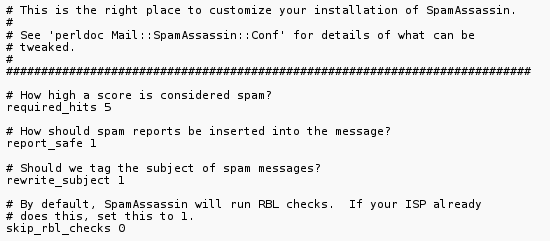
\includegraphics[width=\textwidth]{./annexes/local_sample.png}
 % local_sample.png: 0x0 pixel, 300dpi, 0.00x0.00 cm, bb=
 \caption{Exemple de configuration basique de SpamAssassin}
 \label{fig:local_sample}
\end{figure}
\pagebreak
\subsection{Les règles}
\paragraph{Explications des règles de filtrage de SpamAssassin}
\textbf{SpamAssassin} est basé sur un système de filtrage par règles appliqués lors de tests. 
Ces règles peuvent se mettre dans le fichier de configuration principal (/etc/spamassassin:local.cf) pour 
une configuration globale.
Ce sont ces règles qui vont être vérifiés à chaque message transmis à SpamAssassin, et être utilisés pour les test.

Certaines sont configurés par défaut et permettent de
bien repérer les SPAMs dans la majorité des cas. Cependant pour permettre aux utilisateurs de répondre à des besoins spécifiques,
il est possible d'en déterminer sois même.
\linebreak
Avant d'expliquer les règles en détails, voici un exemple de configuration de règles destinés à la langue Française:
\begin{tiny}
\lstset{numbers=left}
\begin{lstlisting}[language=perl,frame=L,breaklines=true]
#####################################################################################
##### FRENCH SPECIFIC SPAMASSASSIN RULES. 
##### USE AND REDISTRIBUTE WITH THIS NOTE AT YOUR OWN RISK AND PLEASURE.
##### AUTHOR: John GALLET
##### Version: 2008-JUNE-21
##### Latest: http://www.saphirtech.fr/
##### Status: It Works For Me (tm)
#####################################################################################
# Spam is legal in France !
body FR_SPAMISLEGAL                     /\b(Conform.+ment|En vertu).{0,5}(article.{0,4}34.{0,4})?la loi\b/i
describe FR_SPAMISLEGAL                 French: pretends spam is (l)awful.
lang fr describe FR_SPAMISLEGAL		Invoque la loi informatique et libertes.
score FR_SPAMISLEGAL                    2.5

body FR_SPAMISLEGAL_2                   /\bdroit d.acc.+s.{1,3}(de modification)?.{0,5}de rectification\b/i
describe FR_SPAMISLEGAL_2               French: pretends spam is (l)awful.
lang fr describe FR_SPAMISLEGAL_2	Invoque le droit de rectification cnil.
score FR_SPAMISLEGAL_2                  2.5

#####
# yeah, sure.
body FR_NOTSPAM                         /\b(ceci|ce).{1,9} n.est pas.{1,5}spam\b/i
describe FR_NOTSPAM                     French: claims not to be spam.
lang fr describe FR_NOTSPAM		Affirme ne pas etre du spam.
score FR_NOTSPAM                        4.0

header FR_MAILER_1                      X-Mailer =~ /(delosmail|cabestan|ems|mp6|wamailer|
phpmailer|eMailink|Accucast|Benchmail)/i
describe FR_MAILER_1                    French spammy X-Mailer
lang fr describe FR_MAILER_1		X-Mailer couramment employe pour des spams en francais.
score FR_MAILER_1                       4.0

header FR_MAILER_2                      X-EMV-CampagneId =~ /.+/
describe FR_MAILER_2                    French spammy mailer header
lang fr describe FR_MAILER_2		X-Mailer couramment employe pour des spams en francais.
score FR_MAILER_2                       4.0

#####################################################################################
##### END FRENCH SPECIFIC SPAMASSASSIN RULES.
#####################################################################################

\end{lstlisting}
\end{tiny}
Dans ce fichier de configuration, on peux voir que l'on peut influer le score selon certains mots présent dans le mail inspecté, comme dans la première règle par exemple, ou les mots "Conformément" ou "En vertu" rapportent 0.5 points au mail. Le mot "article" en rapporte 0.4, et si il y a quelque chose derrière la chaîne de caractère "34.", cela rapporte 0.4 points aussi. Ce qui fait un total de 1.3 points, On peux voir que le score du mail est de 2.5, si le mail est un spam, il n'a qu'une marge de 1.2 points avant d'être considéré comme tel.

Explication de certaine directives présentes. 

En utilisant cette expression régulière, le mail sera filtré si il contient "agra" dans son corps, comme dans "viagra", même si ce mot est "agrafe" ( Le /i ignore la casse) :
\begin{lstlisting}
body LOCAL_DEM_VIAGRA /agra/i  
\end{lstlisting}

On peux modifier l'écriture de l'entête du mail afin de spécifier que ce mail est un spam :
\begin{lstlisting}
rewrite_header Subject ****SPAM STOP*****
\end{lstlisting}

On utilise le filtre bayésien en incluant cette option : 
\begin{lstlisting}
use_bayes 1
\end{lstlisting}

On indique à SpamAssassin qu'il doit effectuer l'apprentissage automatique des spams :

\begin{lstlisting}
auto_learn 1
\end{lstlisting}

On spécifie que l'on veut recevoir des mails qu'en français avec cette option :

\begin{lstlisting}
ok_languages fr <----- Je n'accepte que les mail en Français
\end{lstlisting}

\paragraph{Les tests}

En règle générale un test se décompose de la manière suivante:
\begin{itemize}
 \item Un nom, consistant jusqu'à 22 lettre majuscule, nombre ou underscores.
 \item Une description plus complète, qui est utilisé dans les rapports générés par SpamAssassin, 
 faisant en règle générale une cinquantaine de caractères
 \item Ou effectuer le test dans le message. Le test peut être effectué uniquement dans l'entête du message, 
 dans le corps du message uniquement, les identifiants de ressources unifiés 
 (URN, détails sur Wikipedia\footnote{\href{http://fr.wikipedia.org/wiki/Uniform_Resource_Identifier}{URN}}).
 \item Une description de ce que les test cherche à capturer. Un test peut spécifier:
    \begin{itemize}
     \item Vérifier l'existence d'un entête
     \item Un expression régulière utilisant la syntaxe en PERl (puisque SpamAssasin est écrit en PERL)
     \item Une liste noire de DNS ou envoyer une requête
     \item Une fonction de SpamAssassin à appeler
     \item Des ``Test flags'' qui permettent de déterminer sous quelles conditions le test doit être appliqué, 
     ou d'autres choses exceptionnels.
     \item Un ou plusieurs scores pour le test. Les tests peuvent avoir un unique score qui est utilisé systématiquement
     , ou avoir des scores différents suivants les 4 conditions suivantes:
	\begin{itemize}\label{cond}
	 \item Quand le filtre Bayésien et les tests réseaux ne sont pas utilisés 
	 \item Quand les tests réseaux sont utilisés mais pas le filtre Bayésien
	\item Quand le filtre Bayésien est utilisé mais pas les test réseaux 
	\item Quand le filtre Bayésien et les tests réseaux  sont utilisés
	\end{itemize}
    \end{itemize}
\end{itemize}

\paragraph{Exemple}
\begin{lstlisting}[frame=single]
header FROM_STARTS_WITH_NUMS    From =~ /^\d\d/
describe FROM_STARTS_WITH_NUMS  From: starts with nums

score FROM_STARTS_WITH_NUMS     0.390 1.574 1.044 0.579
\end{lstlisting}

La directive \emph{header} spécifie que le test portera sur l'entête du message, 
\emph{FROM\_STARTS\_WITH\_NUMS} spécifie le nom du test puis suivis du test à effectuer (ici une expression régulière).
La directive \emph{describe} fournit une description lisible humainement.
La directive \emph{score} va déterminer le score à appliquer au mail si le test s'avère positif. Dans ce cas ci
le score va correspondre aux 4 conditions définit juste au dessus ( Voir au dessus \ref{cond} ). Si cette directive n'est definit qu'avec
un score, il sera appliqué quelque sois la condition.

SpamAssasin est fournis par défaut avec certains tests. Ces tests sont regroupés par type dans des fichiers contenant les règles (ruleset), le score de chaque test 
étant regroupé dans un seul fichier. Ils sont stockées par défaut dans \emph{/usr/share/spamassassin}. On peut
a jouter d'autres ``canaux'' distribuant des règles, grâce à sa-update. Cette fonction automatise la mise
à jour des règles de SpamAsassin. Par défaut seulement \emph{updates.spamassassin.org} est définit comme canal
(ses règles sont mis à jour à chaque nouvelle version). En appelant \emph{sa-update}, toute les règles 
des canaux ajoutés seront mis à jour. Cela permet de tenir automatiquement ses règles à jours au besoin.

\paragraph{modifier le score}
Il est possible de modifier le score d'un test déjà présent par défaut.
Il suffit de rajouter la directive et le nom du test dans le fichier \emph{ /etc/spamassassin/local/.cf}.Exemple:\linebreak
\begin{lstlisting}
score NOM\_TEST 3
\end{lstlisting}
Va changer le score du test \emph{NOM\_TEST} à la valeur 3. On peut faire la même manière pour modifier 
la description d'un test.
\subsection{Fonctionnement de Liste blanche automatique(AWL)}

Quand cette option est activée, SpamAssassin va garder automatiquement une base de données contenant les IPs des expéditeurs des courriers reçus ainsi 
que leurs adresses IPS (ou l'adresses IP du relais ayant transmis le mail). Chaque fois qu'un message est reçu, le score SPAM du message 
est ajouté au score total de l'expéditeur stocké dans la base de donnée, et le nombre de messages reçu de la part de
cet utilisateur est incrémenté. 

Cette fonctionnalité sert surtout à éviter les faux positifs(Un expéditeur régulier ne va pas se mettre subitement à envoyer un SPAM)

Le score moyen d'un expéditeur(score total divisé par le nombre de messages) est utilisé pour modifier  
le score SPAM des nouveaux messages reçu de la part de cet expéditeur. Plus précisément, la différence entre le score 
moyen de l’expéditeur et celui du nouveau message est multiplié par un facteur qui est paramétrable,
et le résultat est ajouté au score du nouveau message. Dans ce cas, quand un nouveau message à son SPAM score 
au dessous de la moyenne, son score SPAM est augmenté, et inversement quand le score SPAM est supérieur à la moyenne
son SPAM score est diminué.

Les test de la liste blanche automatiques sont les derniers exécutés par SpamAssassin, puisqu'il est nécessaire de disposer du score du message.
Egalement, le score moyen de l'expéditeur est mis a jour avant le test avec le SPAM score du message, 
avant que ce score ne soit modifié par la suite.

\subsubsection{Paramétrage de l'AWL}
Le choix important à faire est est de déterminer quel poids l'on va donner à l'historique de l'expéditeur et son score moyen, et celui du SPAM score des messages.
La règle \emph{auto\_whitelist\_factor} va nous permettra de définir le coefficient(un réel) à appliquer. La valeur de ce coefficient 
varie de 0 à 1. Il est par défaut de 0.5, ce qui va mettre le score final appliqué au message entre le score moyen 
de l'expéditeur et celui du message. 

Pour donner plus d'importance au score moyen de l'expéditeur on va augmenter ce coefficient. Quand ce coefficient 
est mis à 1, le score moyen de l'expéditeur va devenir celui du message.



\section{Utilisation }


SpamAssassin peut être utilisé avec des Mail Transfert Agent comme Postfix. On peut par exemple contrôler les messages
avec SpamAssassin juste après leurs réception par le demon SMTPD. Mais la façon la plus répandue est d'utiliser le MDA qui se charge
de filtrer statiquement les mails et de les déposer dans leurs boites mails respectives. 

\subsection{MDA}

Souvent couplé avec \emph{Postfix} (Le serveur de messagerie le plus utilisé dans le monde), procmail est le 
Mail Delivery Agent(Egalement connu comme Local Delivery Agent, sont des programmes qui sont responsable
de la délivrance des mails dans les boites des utilisateurs) que l'on trouve par défaut sur beaucoup de systèmes UNIX.
L'utilisation avec procmail est assez simple. Il faut modifier ou créer le fichier procmail.c qui se trouve dans le répertoire \emph{/etc.}.
Ainsi tout les messages passeront par SpamAssassin avant d'être délivré par procmail. 
\linebreak
Un exemple de procmailrc minimale pour utiliser SPAM assassin:
\begin{lstlisting}[frame=single]  
DROPPRIVS=yes

LOGFILE=/var/log/procmail.log
VERBOSE=ON

# appel du deamon SpamAssassin
| /usr/bin/spamc -f

 :0e
{
   EXITCODE=$?
}
\end{lstlisting}
On peut tout à fait remplacer \emph{spamc} par \emph{spamassassin}. La seul différence étant au niveau des performances, 
chaque appel à la commande \emph{spamassassin}créant un processus distinct, alors que \emph{spamc} fait appel au demon \emph{spamd}.
A partir de là tout va passer à travers SpamAssassin.
\pagebreak

\subsection{SMTP}

Filtrer les mail à l'entré est aussi possible. 
        

\part{Autour de SpamAssasin}

\section{Interfaces graphiques}

Certains solutions graphiques (pour la plupart web) ont intégré SpamAssassin, pour en permettre une administration plus intuitive.
On peut citer notamment:
\begin{description}
 \item 
\end{description}


\section{Plugins non offciels}

Par défaut SpamAssassin intègre plusieurs plugins (modules perl). Mais du fait que c'est un logiciel libre et que son code soit accessible plusieurs
plugins non officiels ont vu le jour. Cette avantage fait que les utilisateurs peuvent créer eux même leurs plugins,
ajoutant ainsi des fonctionnalités à leurs propres solutions intégrant SpamAssassin. Cela inclut également les plugins commerciaux(Plugins utilisant des licences non-libres pour la majorité). 
Parmi ces plugins on peut citer:

\paragraph{Plugin gratuit}
\begin{description}
 \item [DSPAM]Quand DSPAM (antispam léger qui travaille directement sur les connexion SMTP, fait partis du projet open BSD) est utilisé en conjonction avec amavisd-new
 (Qui fait office d'interface entre un MTA et plusieurs gestionnaire de contenus)ce dernier a DSPAM qui calcule automatiquement
 la probabilité que un message est un HAM/SPAM, et de positionner des entêtes. Ce plugin permet de faire prendre en compte 
 ces entêtes pour le score des mails.
 \item [Bayes OCR Plugin] Même méthode que le filtre Bayésien intégré mais qui cette fois s'effectue sur des images en effectuant une reconnaissance 
 optique de caractères (ROC ou OCR en anglais). cela sert à detecter les SPAM envoyer sous forme d'images.
 \item[Image cerberus] Même but que le précédent en analysant les images et en utilisant des techniques de reconnaissances de pattern
 \item[SaveHits]Stocke une copie d'un message dans un répertoire daté quand des règles spécifiques 
 sont atteintes, il créé ensuite un repertoire pour chaque règle contenant un lien symbolique du message.
 Cela permet de rapidement trouvé un message par date correspondants à certaines règles. Utile pour le développement de règles.
 \item [DecodeShortURLs] Ce plugin décode les URL raccourcis en effectuant une requête \emph{HTTP HEAD} au service de raccourcissement d'URL.
 puis l'ajoute à la liste des URL extraites par SpamAssassin , pour que d'autres plugins puissent y avoir accès.
 \item [DNSWL spam reporting] Ajoute le service \emph{DNSWL} aux services qui reçoivent des signalements de SPAM
 grâce à la commande  "spamassassin --report" .
 \item [SAGrey]  Ce plugin est un outil de greylist, qui s’exécute en deux phases.Son but est de permettre 
 de repérer les SPAM uniques. Il effectue deux donc deux vérifications:
 \begin{itemize}
  \item Il vérifie si le score SPAM du mail dépasse le seuil définie
  \item Si c'est le cas il va également vérifié si l’expéditeur est présent dans la liste banche automatique(AWL)
  Si le message dépasse le seuil et n'est pas dans la liste blanche, il va le considérer comme SPAM unique et augmenté le score du mail.
  Il peut également placer ses propres entes. Les avantages de ce module sont de réduire les mails à temporiser dans le cas de greylisting,
  et de ne pas augmenter la taille des bases regroupant les expéditeurs connus. Il est surtout utilisé 
  avec de très grosses architectures mails.
 \end{itemize}

 \item [MTX] Une liste blanche de DNS distribuées. SpamAssasin peut accéder directement à liste.
 \end{description}
\paragraph{Plugin commerciaux}
SpamAssassin peut très facilement ajouter des modules pour augmenter son efficacité. Mais étant donné 
que ce sont des programmes distincts ne faisant que s'interfacer avec SpamAssassin, cela
autorise le développement de plugin propriétaires pour un usage commercial. Les plus connus sont les suivants:
\begin{description}
 \item [Commtouch Plug-in] La société \emph{commtouch} fournit un plugin qui permet d'utiliser les propres technologies
 et antispam de cette dernière. Les messages passe à travers le ``commtouch engine'' et le résultat est convertit en score SpamAssassin.
 Ce plugin permet d'intégrer facilement les fonctionnalités des solutions de la société dans SpamAssassin, de réduire 
 sa maintenance . Il permet egalement de doter facilement SpamAssasin d'un antivirus Zero-Hour(=Qui détecte les virus avant qu'ils ne soient actifs),
 ainsi que renforcer la détection des SPAMs généré par des zombies ou botnet.
 La licence est de type souscription annuelle.Ce plugin est non-libre. 
 Plus d'information sur le \href{http://blog.cyren.com/articles/spamassassin-what-it-is-how-commtouchs-plug-works-with-it-1407.html}{blog} de la société.
 \item[PhishPatrol] Ce plugin fournit par la société Wombat Security Technologies, Inc est dédié au phishing (hameçonnage en français \footnote{Détails sur \href{http://fr.wikipedia.org/wiki/Hame\%C3\%A7onnage}{wikipedia}}
 mais permet aussi une détection du spear phhishing \footnote{Variante plus élaborée du phishing. Voir sur \href{http://fr.wikipedia.org/wiki/Spear_phishing}{wikipedia}}.
 Il fonctionne avec des technologies et services propriétaires fournis par la société. Il vise une intégration homogène avec SpamAssassin.
 Sa licence est non-libre, de type souscription annuelle.
 \item[SNF4SA] Abréviation de ``Message Sniffer Antispam Plugin for SpamAssassin'', ce plugin combine un système collaboratif de réputation
 d'IPs, des technologies d’algorithmes auto-apprenants distribués(distributed competitive machine learning technologies),
 et un moteur d'analyse de contenu qui améliore la précision et la vitesse de SpamAssin, sans modifications additionnels.
 Sa licence est non-libre, ce type souscription commercial.
\end{description}


\section{Solutions pouvant tirer parti des capacités de SpamAssassin}
Les principaux logiciels avec lesquels SpamAssassin doit être couplé pour tirer profit du maximum de ses capacités sont évidemment les clients/serveurs de messagerie, comme par exemple :

\subsection{Au travers de MTA}
\begin{description}
\item [Procmail]
\item [qmail]
\item [sendmail]
\item [Exim]
\end{description}
\subsection{Au travers de MUA}
\begin{description}
\item [Thunderbird]
\item [kmail]
\item [Evolution]
\end{description}

\subsection{SMTP}
\subsection{Et plus encore}
Mais SpamAssassin peut aussi se coupler a d'autres logiciels anti-spam pour obtenir un meilleur résultat de filtrage. On peux notamment l'associer à SpamPal, mais le logiciel anti-spam auquel il est le plus souvent couplé est Bogofilter car il reste le concurrent le plus performant sur ce plan. Bien configurés, l'alliance des deux logiciels permet un filtrage quasi-optimal.\\
Il existe aussi des solutions qui travaillent en commun avec SpamAssassin afin d'améliorer la qualité de leur offre, quelques exemples :
\begin{itemize}
\item [amavisd-new] : Interface entre MTA, scanner de virus et SpamAssassin.
\item [ClearOS] : Serveur Linux pour petites entreprises.
\item [mxHero] : Solution de test de la sécurité du système de mail.
\item [ClamAV] : Solution anti-virus qui peut-être associé a SpamAssassin pour une utilisation optimale.
\end{itemize}

\subsection{Solutions commerciales incluant SpamAssassin}
L'efficacité de SpamAssassin est telle que le logiciel est souvent inclut dans des solutions complètes d'administration système. En voici quelques unes : 
\begin{description}
\item [Parallels Plesk] : Outil permettant de gérer des comptes utilisateurs, noms de domaines, comptes mails, qui inclut SpamAssassin dans sa solution commerciale.
\item [AllEmail] : Proxy POP3 / POP3S utilisant SpamAssassin pour le filtrage anti-spam.
\item [Blacknight] : Offre de passerelle pour les entreprises qui propose SpamAssassin dans leur services.
\item [CleanMail Hosted Anti-Spam] : Solution anti-spam spécialisée Microsoft Exchange, Imail et Lotus.
\item [Antispam.ie] : Solution de filtrage qui élimine le spam avant son entrée dans le réseau du destinataire.
\item [ContentCatcher] : Solution de filtrage personnalisable à but professionnel.
\item [CronLab Anti-Spam Hardware Appliances and Hosted Solution] : Solution complète de management de boite mail.
\item [Heluna] : Solution low-cost pour PME de filtrage.
\item [Spam Interceptor] : Solution anti-spam fonctionnant sur n'importe quel système possédant un navigateur.
\end{description}

SpamAssassin est présent dans bien d'autres solutions, ceci n'était qu'une légère énumération des nombreuses solutions incluant SpamAssassin.

\end{document}

